\section{Experiments}
\label{sec:experiments}

We evaluate seven methods across two spurious-correlation benchmarks
and a controlled mechanism check: Vanilla SGD, our 1st- and 2nd-order
Fairds variants, a corrected 1-step bi-level meta-learner
(\citealt{ren2018reweight}, FORML proxy), JTT \citep{liu2021jtt},
GroupDRO \citep{sagawa2020groupdro}, and IRM \citep{arjovsky2019irm}.
Methods divide into three regimes by the supervision they require:
(i) \emph{no group label at training}: Vanilla, Fairds-1/2, Ren2018,
JTT; (ii) \emph{group label at training}: GroupDRO, IRM; the
fairds variants and Ren2018 use a small group-balanced anchor for
inner-loop computation only.

\subsection{Colored MNIST: where Fairds-2 wins}
\label{sec:exp:cmnist}

\paragraph{Setup.}
We use the IRM-style Colored MNIST setup of \citet{arjovsky2019irm}.
Binary task ($y = \mathbf{1}\{\mathrm{digit} \geq 5\}$); the colour
channel is correlated with the label with probability $0.9$ in the
majority training group, $0.5$ in the minority group, and \emph{flipped
to $0.1$ at test time} (so models that latched onto colour collapse).
Train: 5{,}000 samples, 90:10 majority:minority split.
\textbf{Anchor used inside training algorithms}: 200 samples, 50:50
group-balanced. \textbf{Held-out val\_eval} (never used during training):
500 samples. \textbf{OOD test}: 5{,}000 samples; the worst-group metric
is computed on the (colour $\neq$ label) subset.

We use a small CNN, 10 seeds, 20 epochs. Per-method learning rate is
selected by maximising val\_eval worst-group accuracy (held-out, never
sees test) over $\{0.005, 0.01, 0.02, 0.05\}$; the best $\eta$ is $0.05$
for every method, so the comparison is at matched scale.

\paragraph{Results.}
Table~\ref{tab:cmnist_extended} reports held-out val\_eval and OOD test
metrics for all seven methods. Three observations:

\begin{enumerate}[leftmargin=1.2em, itemsep=2pt, topsep=3pt]
\item \textbf{Fairds-2 substantially improves worst-group accuracy over
Vanilla and over Ren2018} ($+13$~pp / $+2.7$~pp test\_worst,
paired $p\!=\!5\!\times\!10^{-5}$ / $0.052$).
\item \textbf{The 2nd-order cross-term provides an isolated benefit over
the 1st-order alone} (Fairds-2 vs Fairds-1: $+4.7$~pp test\_worst,
paired $p\!=\!0.033$). This is the central mechanism evidence and the
core claim of the paper.
\item \textbf{Stronger baselines exist.} JTT (no group label, 2-stage
ERM) achieves $0.878$ test\_worst, beating Fairds-2 by $+5.4$~pp
($p\!=\!0.032$); GroupDRO (uses group labels at training) achieves
$0.900$, beating Fairds-2 by $+7.6$~pp ($p\!=\!9\!\times\!10^{-5}$).
IRM diverges in our setup. Fairds-2 is therefore not state-of-the-art;
its value is the closed-form, single-pass cross-term mechanism, not
peak worst-group accuracy.
\end{enumerate}

\begin{table}[t]
\centering\footnotesize
\begin{tabular}{llcccc}
\toprule
Method & Family & Group label? & val\_eval\_worst & test\_acc & test\_worst \\
\midrule
Vanilla & — & no & 0.802 $\pm$ 0.068 & 0.716 $\pm$ 0.066 & 0.694 $\pm$ 0.064 \\
\textit{Fairds-1} & closed-form & no & 0.842 $\pm$ 0.057 & 0.791 $\pm$ 0.069 & 0.777 $\pm$ 0.071 \\
\textit{Fairds-2} & closed-form & no & 0.878 $\pm$ 0.034 & 0.836 $\pm$ 0.039 & 0.824 $\pm$ 0.043 \\
FORML & bi-level & no & 0.878 $\pm$ 0.020 & 0.813 $\pm$ 0.048 & 0.796 $\pm$ 0.054 \\
JTT & 2-stage ERM & no & 0.921 $\pm$ 0.030 & 0.886 $\pm$ 0.052 & 0.878 $\pm$ 0.058 \\
\textbf{GroupDRO} & minimax & yes & \textbf{0.922 $\pm$ 0.016} & \textbf{0.906 $\pm$ 0.014} & \textbf{0.900 $\pm$ 0.015} \\
IRM & penalty & yes & 0.590 $\pm$ 0.059 & 0.427 $\pm$ 0.139 & 0.386 $\pm$ 0.160 \\
\bottomrule
\end{tabular}
\caption{\textbf{Colored MNIST extended baselines} (mean $\pm$ std,
10 seeds, best-tuned $\eta$). \textit{Italics} = our methods.
\textbf{Bold} = best in column. Higher is better.}
\label{tab:cmnist_extended}
\end{table}

\begin{table}[t]
\centering\footnotesize
\begin{tabular}{lccc}
\toprule
Method (vs Fairds-2) & $\Delta$ test\_worst & $t$ & $p$ (one-sided $>$) \\
\midrule
Vanilla & -0.1302 & -6.53 & 1 $\downarrow$ \\
Fairds-1 & -0.0465 & -2.08 & 0.967 $\downarrow$ \\
FORML & -0.0272 & -1.81 & 0.948 \\
JTT & +0.0541 & 2.12 & 0.0315 $\uparrow$ \\
GroupDRO & +0.0764 & 6.10 & 8.96e-05 $\uparrow$ \\
IRM & -0.4376 & -8.84 & 1 $\downarrow$ \\
\bottomrule
\end{tabular}
\caption{\textbf{Paired tests vs Fairds-2} (one-sided, same seed).
JTT and GroupDRO are stronger; Vanilla and Fairds-1 are weaker.}
\label{tab:cmnist_pairwise_f2}
\end{table}

\subsection{Mechanism probe on a controlled spurious-feature MLP}
\label{sec:exp:e1b}

To probe whether Fairds-2's gain is consistent with the cross-term
mechanism we hypothesise --- penalising majority-group gradients aligned with
$H_{\mathrm{val}}$'s dominant directions --- we construct a small
controlled regime: a 2-layer MLP, 8-dim feature, 2 classes, with a
single spurious feature that is $\mathcal{N}(\pm 10, 0.3)$ in the
majority group (perfectly label-correlated) and $\mathcal{N}(0, 0.3)$
in the minority group (uncorrelated). Class separation in the
non-spurious dimensions is intentionally weak (only 2 of 8 dimensions
informative), so vanilla MLP must rely on the spurious feature.

\paragraph{Result.}
At majority ratio $0.9$ across 5 seeds, the per-sample $\phi_i$
distributions for Fairds-2 yield Mann--Whitney $U(\mathrm{maj} <
\mathrm{min}) = 1.89\!\times\!10^{-8}$, i.e.\ majority samples receive
significantly \emph{lower} Shapley values than minority samples ---
\emph{supporting} the predicted mechanism. (We caveat that pooling
per-sample $\phi_i$ across seeds risks pseudo-replication; the seed-level
mean of $\Delta\phi$ is also negative for fairds-2 at this ratio.) The
mean per-group $\phi_i$ is monotonically decreasing with imbalance
(Figure~\ref{fig:e1b}): at ratio $0.50$,
$\Delta\phi(\mathrm{maj}-\mathrm{min}) = +0.002$; at ratio $0.99$,
$-0.025$. The 1st-order variant shows the same direction but with a
smaller effect; this is consistent with the test-worst isolation we
observed in Section~\ref{sec:exp:cmnist}.

\begin{figure}[t]
  \centering
  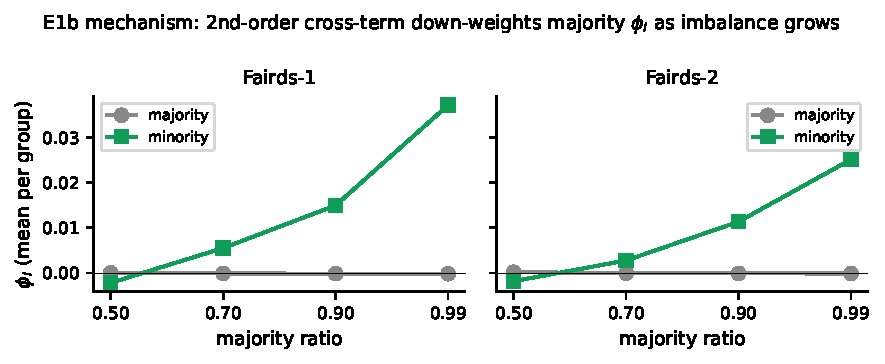
\includegraphics[width=0.9\textwidth]{figures/fig_e1b_phi.pdf}
  \caption{\textbf{Mechanism (E1b).} Mean per-sample $\phi_i$ in the majority
  vs minority group across imbalance ratios on the controlled
  spurious-feature MLP. Both Fairds variants down-weight majority
  $\phi_i$; the 2nd-order cross-term amplifies the effect.}
  \label{fig:e1b}
\end{figure}

\subsection{Waterbirds: where Fairds-2 fails (and why we report it)}
\label{sec:exp:waterbirds}

\paragraph{Setup.}
We evaluate on the canonical Waterbirds benchmark
\citep{sagawa2020groupdro}: bird species (waterbird vs landbird)
with background (water vs land) as a strong spurious feature. We use
ResNet-18 pretrained on ImageNet (BN running stats frozen for
vmap compatibility), 4{,}795 training images, anchor of 200 (50 per
group balanced), 999 held-out val\_eval, 5{,}794 OOD test (4 group
breakdown). 3 seeds, 10--15 epochs.

\paragraph{Three algorithmic variants.}
Anticipating that the EMA buffer might accumulate noise from small
fine-tuning gradients, we tried three Fairds variants:
(a) default EMA with strong reweighting
($\tau\!=\!0.1, w_{\mathrm{scale}}\!=\!4$);
(b) default EMA with \texttt{warmup\_epochs}$=3$ (vanilla SGD for the
first three epochs, Fairds afterwards);
(c) \texttt{no\_ema} per-step weighting with $\eta\!=\!10^{-4}$ and
\texttt{warmup\_epochs}$=1$ for 15 epochs.

\paragraph{Result.}
All three variants of Fairds-2 fail to match the bi-level baseline
(Table~\ref{tab:waterbirds_grid}). Variant (a) is \emph{below} vanilla
(catastrophic). Variant (b) brings parity with vanilla. Variant (c)
marginally beats vanilla ($+7$~pp, $p\!=\!0.17$, not significant) but is
still $\sim\!30$~pp below the corrected Ren2018 baseline (paired
$p\!=\!0.997$, Ren2018 strictly dominates).

\begin{table}[t]
\centering\small
\begin{tabular}{lccc}
\toprule
Method & default-hp & warmup=3 & no\_ema \\
\midrule
Vanilla & 0.182 $\pm$ 0.033 & 0.182 $\pm$ 0.033 & 0.115 $\pm$ 0.064 \\
Fairds-1 & 0.134 $\pm$ 0.095 & 0.180 $\pm$ 0.081 & 0.184 $\pm$ 0.050 \\
Fairds-2 & 0.145 $\pm$ 0.081 & 0.200 $\pm$ 0.086 & 0.189 $\pm$ 0.047 \\
FORML & 0.494 $\pm$ 0.058 & 0.494 $\pm$ 0.058 & 0.499 $\pm$ 0.081 \\
\bottomrule
\end{tabular}
\caption{\textbf{Waterbirds OOD test\_worst} across three Fairds variants
(mean $\pm$ std, 3 seeds). Higher is better. Fairds variants do not
approach Ren2018; the regime-boundary diagnosis is in
Section~\ref{sec:discussion}.}
\label{tab:waterbirds_grid}
\end{table}

\paragraph{On Adult/COMPAS.}
A pareto-style hyperparameter sweep on UCI Adult shows that the
Pareto front in (val acc, dp\_diff $+$ eo\_diff) is jointly spanned
by Vanilla and Ren2018; Fairds-2 is dominated. A 17$\times$ sweep of
the per-batch weight magnitude does not move Fairds-2 onto the
front, ruling out a ``weights are too small'' explanation. Details
in Appendix~\ref{app:e2}. Wall-clock overhead measurements are in
Appendix~\ref{app:overhead}.
